% This is samplepaper.tex, a sample chapter demonstrating the
% LLNCS macro package for Springer Computer Science proceedings;
% Version 2.20 of 2017/10/04
%
\documentclass[runningheads]{llncs}
%
\setlength{\arrayrulewidth}{0.25mm}
\setlength{\tabcolsep}{10pt}
\renewcommand{\arraystretch}{1.5}
\usepackage{graphicx}
\usepackage{caption}
\usepackage{subcaption}
\graphicspath{{figures/}}
% Used for displaying a sample figure. If possible, figure files should
% be included in EPS format.
%
% If you use the hyperref package, please uncomment the following line
% to display URLs in blue roman font according to Springer's eBook style:
% \renewcommand\UrlFont{\color{blue}\rmfamily}

\begin{document}
%
\title{Forecasting Energy Consumption in the Philippines Using Machine Learning Algorithms}
%
\titlerunning{Forecasting Energy Consumption in the Philippines}
% If the paper title is too long for the running head, you can set
% an abbreviated paper title here
%
\author{Erru Torculas \and
Earl James Rentillo \and
%Brethren Ace de la Gente \and
Ara Abigail Ambita}
%
\authorrunning{E. Torculas et al.}
% First names are abbreviated in the running head.
% If there are more than two authors, 'et al.' is used.
%
\institute{Division of Physical Sciences and Mathematics \\ University of the Philippines Visayas \\ Miagao, Iloilo, Philippines \\
\email{\{egtorculas, eqrentillo\}@up.edu.ph}}
%
\maketitle              % typeset the header of the contribution
%
\begin{abstract}
In the Philippines, usage of energy has been steadily increasing over the years, however, the advent of the COVID19 pandemic brought about unforeseen changes to these parameters. By using machine learning algorithms, energy predictions can be more properly assessed, and corresponding measures can be put into place. The Monthly and Quarterly Market Assessment Report of Wholesale Electricity Spot Market(WESM), governed by Philippines Electricity Market Corporation  (PEMC)'s data will be analyzed using three machine learning algorithms, namely: Linear Regression, SVR, and XGBoost to determine the best algorithm in predicting energy consumption within the pre-pandemic and pandemic periods. To compare between algorithms, the metric of choice will be Random Square Mean Error (RSME). Anaconda will be the main tool used in the project, alongside umbrella applications such as Jupyter and Datalore. Python will be the chosen programming language, and packages that are deemed valuable will also be utilized.

\keywords{Energy consumption \and Forecast \and Machine learning}
\end{abstract}
%
%
%
\section{Introduction}
Energy has always played a vital part in modern society. In fact, Barak and Sadegh (2016) introduced how consumption of such a resource exhibits a continuous rise to developing economies. It performs as a societal backbone in that its utilization is deemed essential from fueling activities, from mundane ones up to crucial operations. Exemplified by sectors such as residential, commercial, and industrial using electricity as a primary source for operation, energy consumption\footnote{Github Repository: \url{https://github.com/errutorculas/cmsc197-ML-miniproj}} is thus generally regarded as an index of standard of living (NIOS, 2012).

In the Philippines, the average energy consumption per person reached a peak of 5,205 kWh in 2019 and has been relatively increasing in each year prior. Some notable trends which follow this annual increase include country energy consumption (peaked at 563 TWh in 2019), country electricity generation (peaked at 108.27 TWh in 2021), and average electricity generation per person (peaked at 961 KWh in 2019). 

These statistics, as authored by Ritchie et al. (2019), go to show how studying energy consumption in the Philippines proves to be relevant, especially that the population’s access to electricity is at an all-time high at 96.84\%. Furthermore, Barak and Sadegh (2016) also mentioned how there is a lack of datasets in developing economies to be able to predict future demands in electricity. This is where tools such as regression analysis become useful to bridge the gap of such data deficiency. It can be used to generate predicted data and thus arrive at a plausible conclusion if energy demands would still be met in the years to come. More importantly, knowing the pattern of consumption and predicting the trend of energy consumption can work to determine priorities in the process of taking decisions on a sustainable urban environment for the energy sector in the Philippines, and therefore be a reasonable metric to improve energy efficiency of industrial and commercial industries for better policymaking. 

Finally, accomplishing the mini-project would be beneficial in concretizing findings established in relevant past studies, as well as exploring how these build on in more specific contexts such as of the Philippines. Relatively, this would also be able to help future research, in that it could provide insights from the methodology and findings gathered in regression analysis and thus foreground the generation of more accurate results.

This paper will assess different machine learning algorithms in forecasting time series of energy consumption in the Philippines and compare the viability and accuracy of each forecasting. By this, allowing the researchers to investigate on which approach is likely to be accurate for future implementation of energy consumption prediction.

\subsection{Literature Review}
Shin and Woo (2022) compared three distinct machine-learning algorithms, namely the Random (RF) model, XGBoost (XGB) model, and Long Short-Term Memory (LSTM) model in order to predict the energy consumption of Korea. The researchers concluded their findings by suggesting the applicability of machine learning in forecasting energy consumption. Although there is also an evident demonstration of machine learning being outperformed by traditional econometric approaches,  ML is advantageous and works better when encountered with unexpected irregular time series data ML. 

Similarly, Rambabu et. al. (2022) exhaustively delved into the prediction and analysis of household energy consumption through machine learning algorithms for energy management. Their paper focused on predicting household energy consumption where models are trained by using various machine learning algorithms such as Linear Regression, Lasso Regression, Random Forest, Extra Tree Regressor, XG Boost, etc. It must be noted that patterns of household energy consumption are observed by the constant changing of different factors namely, temperature, humidity, an hour of the day, etc. The researchers’ findings suggested that tree-based models give the best results among the rest of the machine-learning approaches used. This is because they evaluated the models using R square as the forecasting is based on time. R square can be utilized to gauge how much variance in the dependent variable can be predicted. 

A case study in Malaysia discussed energy consumption prediction by using three methodologies of machine learning, specifically, Support Vector Machine, Artificial Neural Network, and k-Nearest Neighbor. These approaches were proposed for the algorithm of the predictive model. Shapi et. al. (2021) explored a great insight into real-life applications where the researchers used two tenants from a commercial building as proponents of their case study. The metrics of evaluation used in the paper are compared based on RMSE, NRMSE, and MAPE metrics.

\section{Data and Methodology}
This chapter presents the data used throughout the paper and describes the implementation method that will be performed to accomplish the project objective. With this, it will also discuss the process of the researchers and the analysis used through evaluation metrics to assess the performance of the models.
\subsection{Data}

\subsubsection{Dataset}~\\

The data used throughout this project is consolidated data\footnote{For reference of the Energy dataset:\\ 
\url{https://drive.google.com/drive/folders/1yxtk9GNx4CCfY3Eh4bY19\_5nwx5HcVbw?usp=share\_link}} from 2014 to the second quarter of 2022 of the Monthly and Quarterly Market Assessment Report of the Wholesale Electricity Spot Market (WESM) governed by the Philippines Electricity Market Corporation (PEMC) \cite{pemc}. Also, the Department of Energy 2020 Summary Power Statistics was also utilized as a basis for Power Consumption by Sector, specifically, the Commercial and Industrial data.

\subsubsection{Data Fields}
\begin{itemize}
    \item \textbf{Year}. Indicating the specific year of the month that the energy consumption data was observed.
    \item \textbf{Month}. Signifies the specific month that the energy consumption data was observed
    \item \textbf{Date}. Complete detail of the year, month, and day that the energy was observed.
    \item \textbf{Total Energy Consumption (in GWh)}. This refers to the sum of monthly energy consumption from January of 2014 up to June 2022. 
    \item \textbf{Total Energy Consumption of CC by Industry Type (in GWh)}. Denotes the energy consumption of Contestatable Customers\footnote{The term is used for a customer that engages in consolidating electric power demand to end-users and is able to choose their own electricity provider} by its Industry type, namely, Commercial and Industrial.
    \item \textbf{Load Factor (in \%)}. An indicator of energy efficiency to describe consumption characteristics of electricity over a period of time.
    \item \textbf{Quarterly Total Energy Consumption (in GWh)}. Observed energy consumption quarterly. Specific months such as March, June, September, and December.  
\end{itemize}

\subsubsection{Caveats}~\\

The data were mostly curated from the summary reports of WESM. So, the total energy consumption data for 2016 is only available through a bar graph without any numeric label accompanying the bar in each month. Estimates were used based on the graph itself. Moreover, the total energy consumption of CC by Industry type column of the dataset, data from the year 2014 to 2017 do not have any available data to include in the dataset. Missing data from the Load Factor from the year 2016 until 2017. With that, no relevant reports pertaining to this are available publicly.

\subsection{Methodology}

To evaluate the data concerning the scope of the project, three machine learning algorithms are run and compared with each other for accuracy. The models that will be implemented in this paper are: \textit{Random Forest (RF) Model, XGBoost, Linear Regression,} and lastly, \textit{Support Vector Regression (SVR)}. These models were selected because they yield a significant analysis and meaningful information in a predictive approach based from the previous published related works. Not only that, this paper revolves on finding the accurate model to implement in terms of forecasting energy consumption therefore regression is advantageous in capturing associations and relationships between forecast variable of interest and predictor variables.

The time periods for analysis are divided into two, namely: Pre-pandemic and Pandemic periods, Period 1 and Period 2, respectively. The separation of time periods serves as the basis of the efficiency of the models when practiced on a sudden shift of regulations brought by the height of the pandemic.

The pre-pandemic period is composed of rather linear growth in terms of energy consumption and saw a rise from a starting point of 4422 GWh (Jan 2014) to an endpoint of 6224 GWh (Mar 2020) and a peak point of 7697 GWh (Jun 2019).

Following this, Period 1 will make use of "January 2014 to March 2020" in which the training data will start from "January 2014 to June 2018", while the rest will be the testing data "July 2018 to March 2020"

One of the main reasons for the group’s undertaking of the project can be seen in the data from April 2020, which was the first month of lockdown and in turn, led to a staggering decrease in energy consumption(3760 GWh from the previous month’s 6224 GWh) as non-essential buildings were cut off to minimize losses, amongst other reasons. Power generation was drastically reduced due to slowdown in terms of economical manufacturing production, and the energy consumption both in commercial and infrastructure sector by 2.0\% \cite{shin-woo}.

Following this, Period 2 uses "January 2014 to February 2020" as the training data, the period wherein it witnessed the drastic change in energy consumption. Meanwhile, the testing data will use "March 2020 to June 2022".

This paper will provide separate models in order to demonstrate their respective predictive performance in accordance to the situation of the market. Overall, the machine learning models mentioned will be made possible because of Python, importing series of statistical package and libraries for empirical analysis later on.

As for the preprocessing, this paper will only involve two dataset field which are the \textit{Date} and \textit{Total Energy Consumption (in GWh)}. In fact, the \textit{Date} will be set and serve as the index of the entire data. Additionally, forecasting will thoroughly engage in time series, hence, \textit{create\_features()} function will create a copy distinguishing the features \textit{"Quarter"}, \textit{"Month"}, \textit{"Year"}, and \textit{"Day of Year"} and aid the training data as some kind of indicators. On the other hand, the target of the implementation is to evaluate the \textit{Total Energy Consumption (in GWh)}. The model will only revolve in a univariate approach, independent (date) and independent (energy consumption) variables.

Initializing the training and testing data, Period 1 and Period 2 will have their own respective set. \textit{trainPre} and \textit{testPre} for Period 1, while, \textit{trainPan} and \textit{testPan} for the pandemic Period 2. With that, both periods will also be accompanied by an independent features \textit{X\_train} and \textit{X\_test}. Also, the target or the dependent variable which is the energy consumption, \textit{y\_train} and \textit{y\_test}.

\subsection{Evaluating Forecast Accuracy}
Since the result of the focus of the project is regression analysis, in the context of prediction driven models, the most widely adopted reliability analysis indicators are Root Mean Square Error (RMSE) and Mean Absolute Percentage Error (MAPE). RMSE measures the differences between the predicted and actual values and therefore a means to measure the quality of fit between the actual data and predicted model. It is preferred over the standard Mean Square Error (MSE) since it is a smaller value and can be compared more straightforwardly. Furthermore, MAPE is one of the metrics of evaluation used in this paper since it relatively measures how accurate the forecast system is. RMSE equation is shown in Equation (1), while the equation of MAPE is shown in Equation (2) \\

\begin{equation}
    RMSE = \sqrt{\frac{\sum_{i=1}^{n}(x_{1,i} - x_{2,i})^2}{n}}  
\end{equation}

\begin{equation}
    MAPE = \frac{1}{n}\sum_{i=1}^{n}\left | \frac{x_{1,i} - x_{2,i}}{x_{1,i}} \right | \times 100
\end{equation}

\section{Philippines Energy Consumption Model}
\subsection{Random Forest (RF) Model}
Random Forest can be applied to time series forecasting by converting the time series data into a format suitable for supervised learning and using a specific method called walk-forward validation to evaluate the model. This is necessary because using k-fold cross validation on the model would produce overly optimistic results.

In the RF model, the hyperparameter for this model was changed. Through the \textit{RandomForestRegssor()} function, the \textit{n\_estimators} were increased from its default value of 1000 to 10000 and \textit{max\_features} to 4. 
\begin{figure}[h]
    \begin{subfigure}[h]{\textwidth}
         \centering
         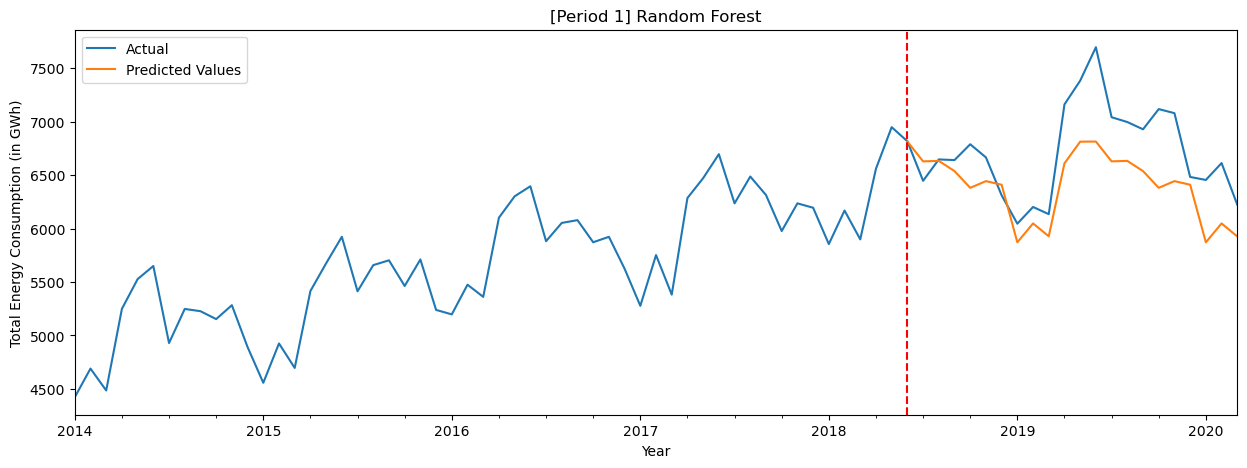
\includegraphics[width=\textwidth]{rf/p1-RF.png}
         \caption{}
         \label{fig:modelRF-p1}
    \end{subfigure}
    \begin{subfigure}[h]{\textwidth}
         \centering
         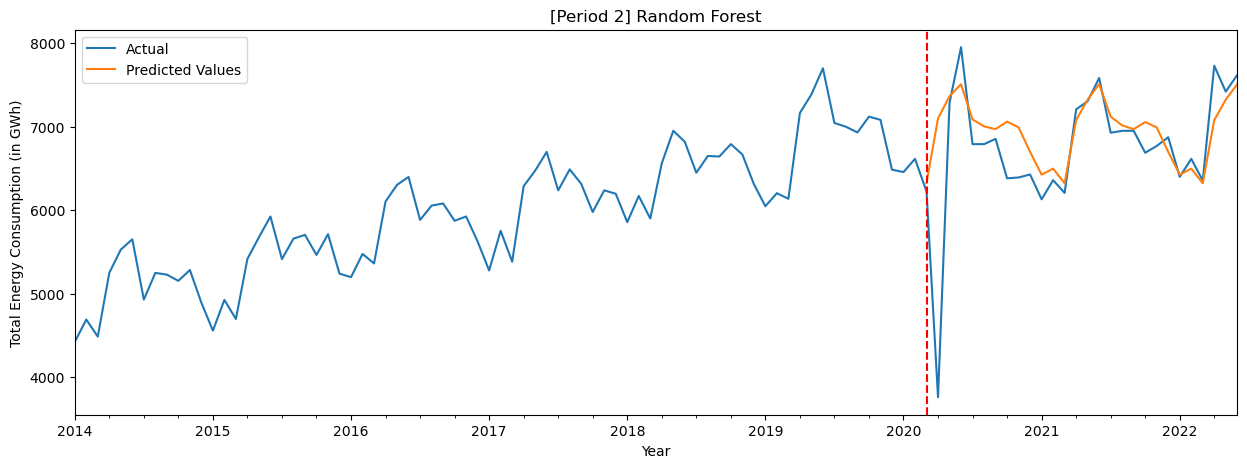
\includegraphics[width=\textwidth]{rf/p2-RF.png}
         \caption{}
         \label{fig:modelRF-p2}
    \end{subfigure}
    \caption{Random Forest Forecasting}
    \label{fig:fig1}
\end{figure}
Training data features were then fitted into the model. In fact, these features comprised of time series and the energy consumption, \textit{X\_train} and \textit{y\_train}, respectively.\\

For both periods, 1 and 2, each respective training sets were fit into the model to garner predicted values. Figure \ref{fig:fig1} below illustrates model of the Random Forest in forecasting energy consumption. The actual and predicted values of the total energy consumption were compared through a graph. Figure \ref{fig:modelRF-p1} depicts the actual and predicted values of Period 1, Pre-pandemic, until March 2020. While Period 2 values were indicated in Figure \ref{fig:modelRF-p2}, until the last recent update in June 2022.


\subsection{XGBoost Model}
XGBoost has been shown to be effective in a variety of tasks, including time series forecasting. It can be able to handle large datasets and a high number of features, which is often in this case where there may be a large number of historical data points and exogenous variables that can be used to make predictions.
\begin{figure}[h]
    \begin{subfigure}[h]{\textwidth}
         \centering
         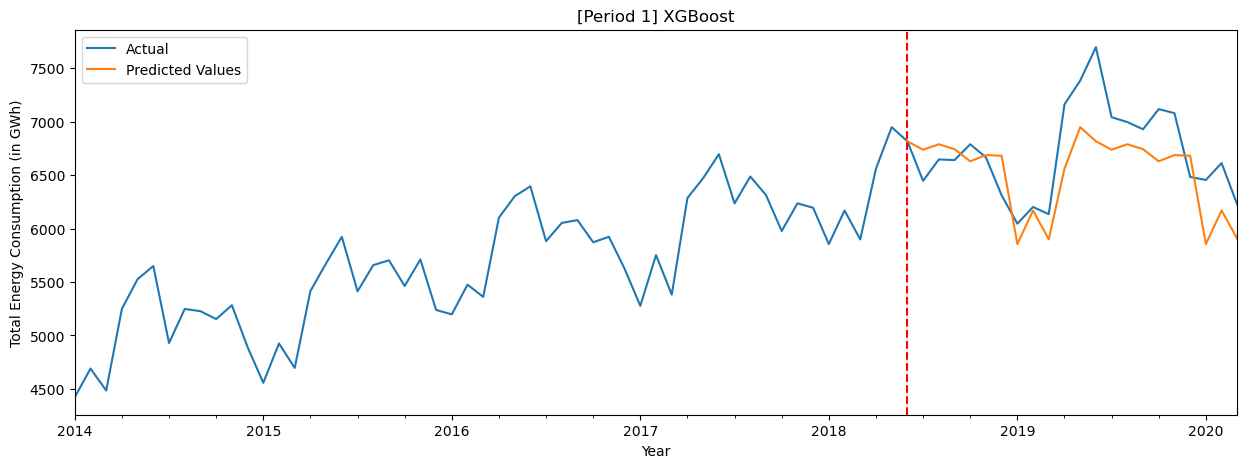
\includegraphics[width=\textwidth]{xgboost/p1-XGBoost.png}
         \caption{}
         \label{fig:modelXGBoost-p1}
    \end{subfigure}
    \begin{subfigure}[h]{\textwidth}
         \centering
         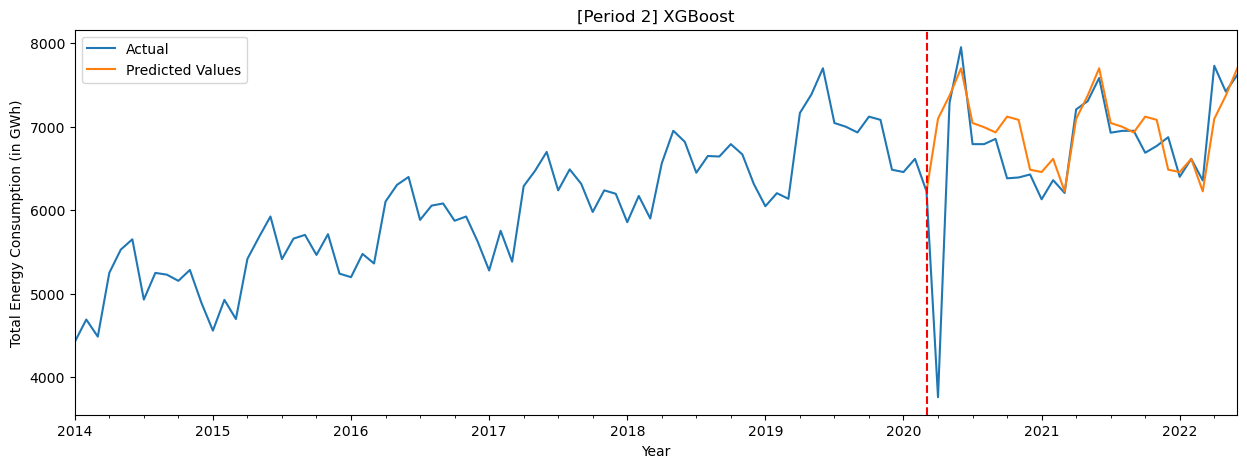
\includegraphics[width=\textwidth]{xgboost/p2-XGBoost.png}
         \caption{}
         \label{fig:modelXGBoost-p2}
    \end{subfigure}
    \caption{XGBoost Forecasting}
    \label{fig:xgboost-model}
\end{figure}

In the XGBoost model, the hyperparameter for this model was changed. \textit{XGBRegressor()} function was used wherein the \textit{n\_estimators} were changed from its default value to 10000. The training data from both periods were fitted using the time series features and total energy consumption. Figure \ref{fig:xgboost-model} illustrates the comparison graph of actual and predicted values for the total energy consumption. 

The figure depicts the actual and predicted values of the total energy consumption through forecasting using the XGBoost model. The model was repeated trained until the RMSE value is minimized. For Period 1 (Figure \ref{fig:modelXGBoost-p1}) and 2 (Figure \ref{fig:modelXGBoost-p2}), in order to decide the final model for the Random Forest with minimal RMSE, repeated training was conducted. Hence, output from Figure \ref{fig:xgboost-model}. 

\subsection{Linear Regression Model}.
\begin{figure}
    \begin{subfigure}[b]{\textwidth}
         \centering
         \includegraphics[width=\textwidth]{lr/p1-lr.png}
         \caption{}
         \label{fig:modelLR-p1}
    \end{subfigure}
    \begin{subfigure}[b]{\textwidth}
         \centering
         \includegraphics[width=\textwidth]{lr/p2-lr.png}
         \caption{}
         \label{fig:modelLR-p2}
    \end{subfigure}
    \caption{Linear Regression Forecasting}
    \label{fig:lr-model}
\end{figure}
Linear regression is a simple but powerful technique for forecasting. It is effective because it makes a strong assumption about the relationship between the input variables and the output variable, which allows it to make reliable predictions even when the data is noisy or there are missing values. In fact, linear regression is fast and easy to implement, making it a popular choice for many forecasting tasks.

In the Linear Regression model, there are no hyperparameters involve for tuning. It fits the linear model that will minimize the difference between the predicted values and the actual values in the data between the observed target which is the total energy consumption. As a result, linear approximation is observed to make predictions about the target variables. Figure \ref{fig:lr-model} illustrates the comparison graph of actual and predicted values for the total energy consumption. 

\subsection{Support Vector Regression (SVR) Model}
\begin{figure}
    \begin{subfigure}[b]{\textwidth}
         \centering
         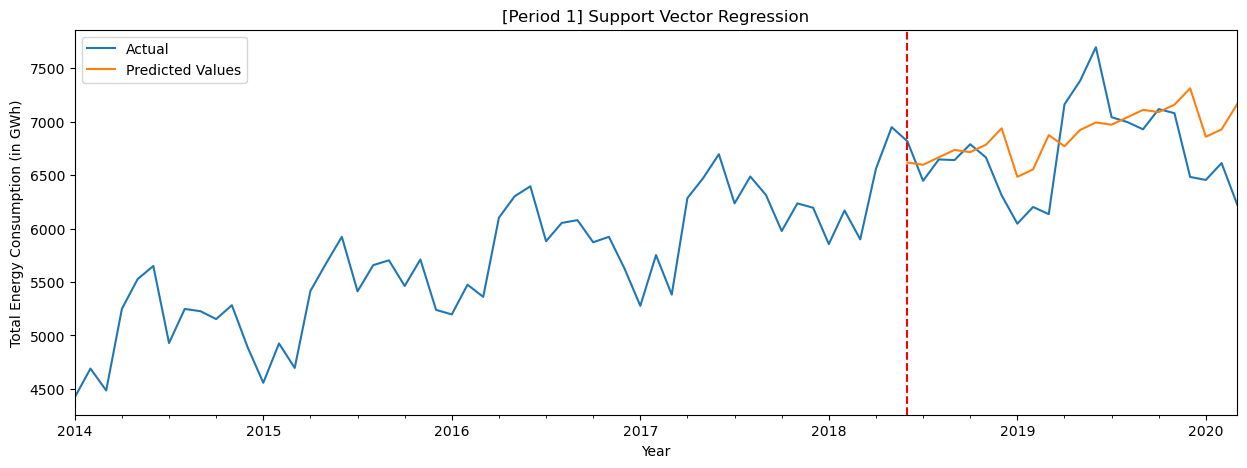
\includegraphics[width=\textwidth]{svr/p1-SVR.png}
         \caption{}
         \label{fig:modelSVR-p1}
    \end{subfigure}
    \begin{subfigure}[b]{\textwidth}
         \centering
         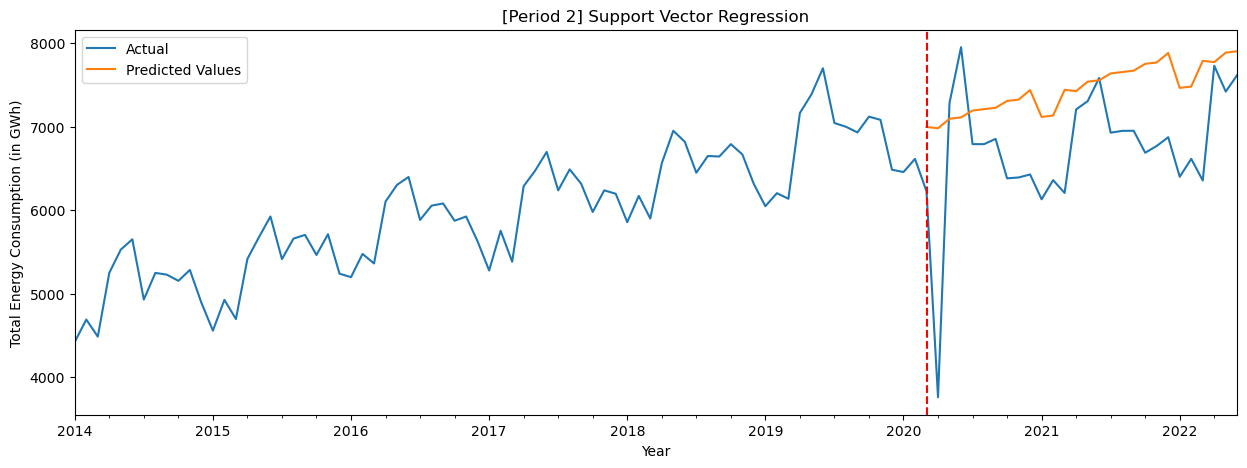
\includegraphics[width=\textwidth]{svr/p2-SVR.png}
         \caption{}
         \label{fig:modelSVR-p2}
    \end{subfigure}
    \caption{Support Vector Regression (SVR) Forecasting}
    \label{fig:svr-model}
\end{figure}
Support Vector Regression (SVR) is a type of support vector machine (SVM) that is often used for regression tasks. It works by finding the hyperplane in a high-dimensional space that maximally separates the data points of different classes. In the case of regression, the classes are continuous, and the goal is to find the hyperplane that best fits the data.

SVR is often used for forecasting because it can handle data with multiple features and can make predictions for continuous target variables. It can also perform well in cases where there is a lot of noise in the data, as it is robust to outliers. Not only that, SVR models can also be trained relatively quickly, making them efficient for use in forecasting tasks.

In the Support Vector Regression (SVR) model, the hyperparameter for this model was changed. \textit{SVR()} function was used wherein the \textit{kernel} value is \textit{linear}, changed the regularization parameter \textit{C} from its default value to 10000, and \textit{epsilon} equal to 10. Both periods were fitted using the time series features and total energy consumption. Figure \ref{fig:svr-model} illustrates the comparison graph of actual and predicted values for the total energy consumption. Overall, in order to decide the final model for the SVR with minimal RMSE, repeated training was conducted. Hence, output from Figure \ref{fig:svr-model}. 

\section{Results}
The group utilized the Scikit learn package to build Random Forest, XGBoost, Linear Regression, and Support Vector Regression models. With that, the final model was chosen based on the lowest root mean squared error (RMSE) value. Table \ref{tab:perf} compares the test data RMSE values of the machine learning models for two different periods, Period 1 and 2.

\begin{center}
\begin{table}[]
    \centering
    \caption{Performance of the models by period}
    \label{tab:perf}
    \begin{tabular}{cccccc}
    \hline
    \multicolumn{4}{r}{\textbf{ML Models}} \\
    \cline{3-6}
      & \textbf{Metric}    & \textbf{RF}    & \textbf{XGBoost}  & \textbf{Linear Reg}    & \textbf{SVR}      \\
    \hline
    \textbf{Period 1}    & RMSE      & 422.737   & 366.691   & 411.578   & 431.366\\
                & MAPE      & 0.050     & 0.044     & 0.047     & 0.050\\
    \hline
    \hline
    \textbf{Period 2}    & RMSE      & 687.665   & 692.077   & 935.880   & 982.202\\
                & MAPE      & 0.061     & 0.061     & 0.123     & 0.131\\
    \hline
    \end{tabular}
\end{table}
\end{center}

The group utilized the Scikit learn package to build Random Forest, XGBoost, Linear Regression, and Support Vector Regression models. With that, the final model was chosen based on the lowest root mean squared error (RMSE) value. Table \ref{tab:perf} compares the test data RMSE values of the machine learning models for two different periods, Period 1 and 2. The group utilized the Scikit learn package to build Random Forest, XGBoost, Linear Regression, and Support Vector Regression models. With that, the final model was chosen based on the lowest root mean squared error (RMSE) value. Table \ref{tab:perf} compares the test data RMSE values of the machine learning models for two different periods, Period 1 and 2.

\begin{figure}[h]
    \begin{subfigure}[h]{\textwidth}
         \centering
         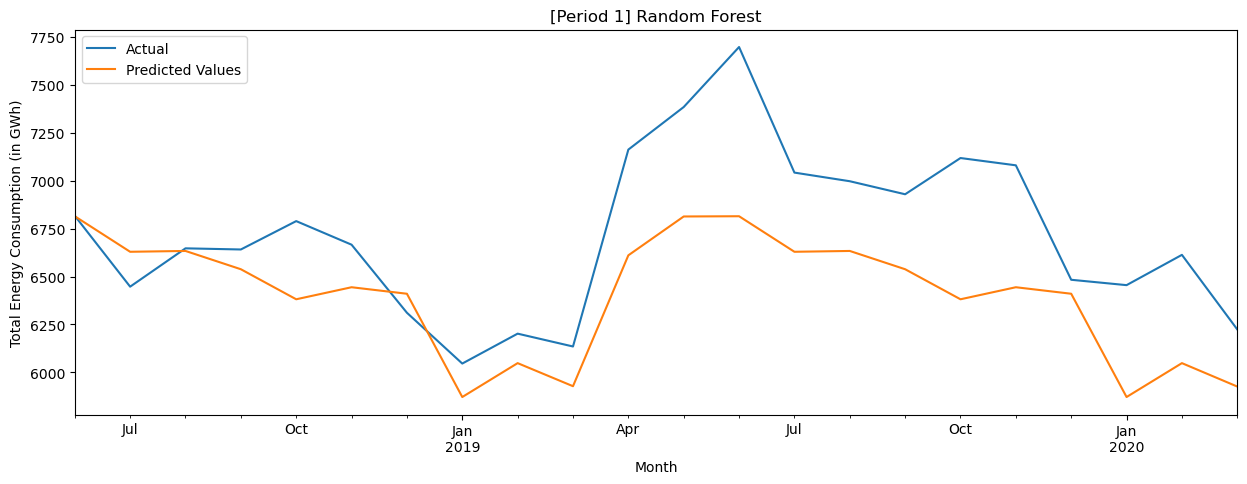
\includegraphics[width=\textwidth]{rf/p1-1-RF.png}
         \caption{}
         \label{fig:modelRF-p1}
    \end{subfigure}
    \begin{subfigure}[h]{\textwidth}
         \centering
         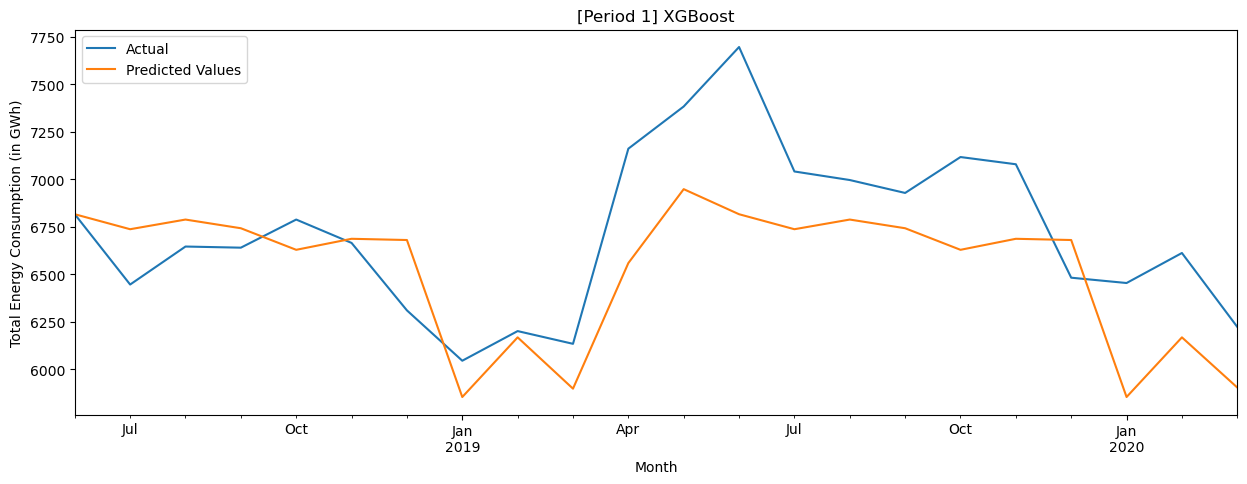
\includegraphics[width=\textwidth]{xgboost/p1-1-XGBoost.png}
         \caption{}
         \label{fig:modelRF-p2}
    \end{subfigure}
    \begin{subfigure}[h]{\textwidth}
         \centering
         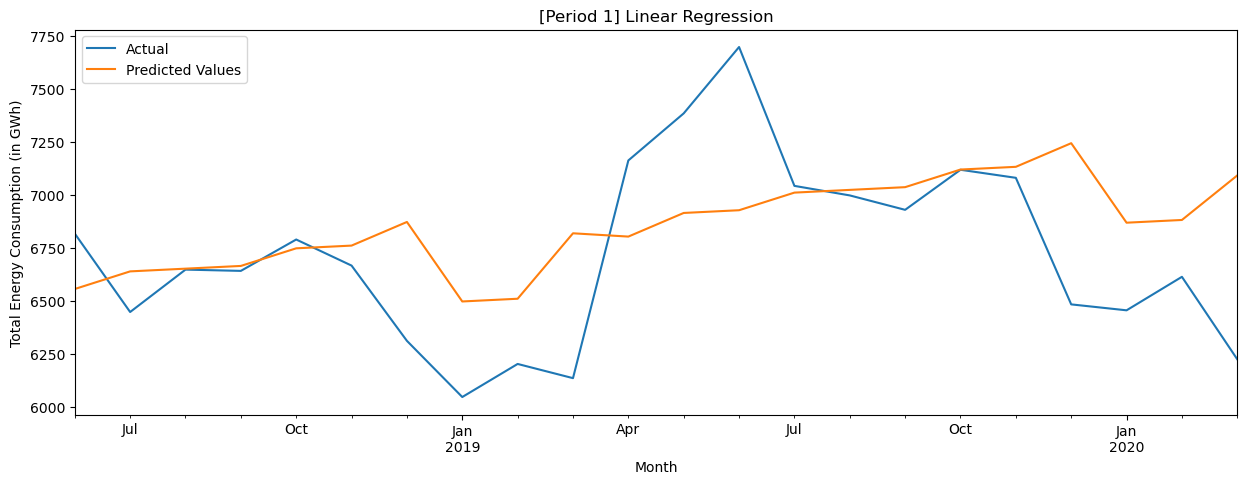
\includegraphics[width=\textwidth]{lr/p1-1-LR.png}
         \caption{}
         \label{fig:modelRF-p1}
    \end{subfigure}
    \begin{subfigure}[h]{\textwidth}
         \centering
         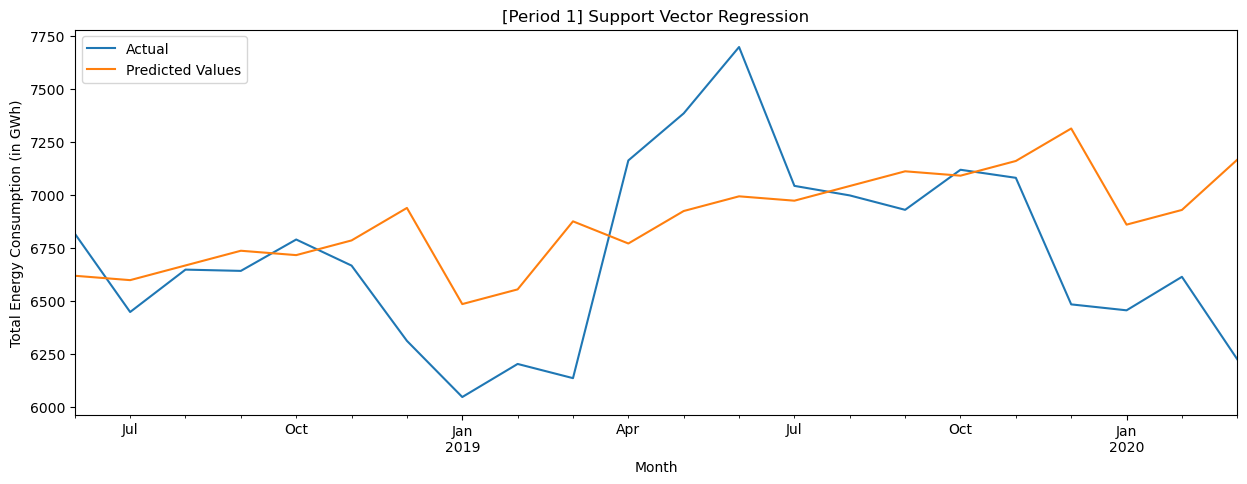
\includegraphics[width=\textwidth]{figures/svr/p1-1-SVR.png}
         \caption{}
         \label{fig:modelRF-p2}
    \end{subfigure}
    \caption{Period 1 Models Forecasting}
    \label{fig:fig1}
\end{figure}

\section{Conclusion}






%
% ---- Bibliography ----
%
% BibTeX users should specify bibliography style 'splncs04'.
% References will then be sorted and formatted in the correct style.
%
% \bibliographystyle{splncs04}
% \bibliography{mybibliography}
%
\begin{thebibliography}{15}
\bibitem{bakrak-sadegh}
S. Barak and S. Sadegh. “Forecasting energy consumption using ensemble ARIMA–ANFIS hybrid algorithm”. In: \textit{International Journal of Electrical Power Energy Systems} 82 (2016).

\bibitem{pemc}
Philippine Electricity Market Corporation. \textit{Monthly Market Assessment Report}. Accessed: 2022-11-27. 2019. URL: \url{https://www.wesm.ph/market- outcomes/market-assessment-reports/monthly-market-assessment- report}.

\bibitem{garcia-martin-estimation}
E. Garcia-Martin et al. “Estimation of energy consumption in machine learning”. In: \textit{Journal of Parallel and Distributed Computing} 134 (2019), pp. 75–88.

\bibitem{shin-woo}
S. Shin and H. Woo. “Energy Consumption Forecasting in Korea Using Machine Learning Algorithms”. In: \textit{Energies} 15.13 (2022).

\bibitem{garcia-martin-measure}
E. Garcia-Martin et al. H\textit{How to Measure Energy Consumption in Machine Learning Algorithms}. Lecture Notes in Computer Science. Cham, Switzer- land: Springer, 2019, pp. 243–255.

\bibitem{kim}
B.-G. Kim et al. “Dynamic Pricing and Energy Consumption Scheduling With Reinforcement Learning”. In: \textit{IEEE Transactions on Smart Grid} 7.5 (2016), pp. 2187–2198.

\bibitem{lemaire}
“European Conference on Machine Learning and Principles and Practice of Knowledge Discovery”. In: \textit{Advanced Analytics and Learning on Temporal Data}. Ed. by V. Lemaire et al. Vol. 1196. Lecture Notes in Artificial Intelligence. Würzburg, Germany: Springer, 2019.

\bibitem{li}
C. Li et al. “Building Energy Consumption Prediction: An Extreme Deep Learning Approach”. In: \textit{Energies} 10.10 (2017).

\bibitem{mosavi-bahmani}
A. Mosavi A. Bahmani. \textit{Energy Consumption Prediction Using Machine Learning; A Review}. Accessed: 2022-11-27. 2019. URL: \url{https://www. preprints.org/manuscript/201903.0131/v1}.

\bibitem{rambabu}
M. Rambabu, N. Ramakrishna, and P.K. Polamarasetty. “Prediction and Analysis of Household Energy Consumption by Machine Learning Algorithms in Energy Management”. In: \textit{E3S Web of Conferences} (2022).

\bibitem{ritchie}
H. Ritchie, Roser M., and P. Rosado. \textit{Philippines: Energy Country Profile}. Accessed: 2022-11-27. Our World in Data. 2022. URL: \textit{https:// ourworldindata.org/energy/country/philippines}.

\bibitem{sahakian}
M. D. Sahakian. “Understanding household energy consumption patterns: When “West Is Best” in Metro Manila”. In: \textit{Energy Policy} 39.2 (2011), pp. 596–602.

\end{thebibliography}
\end{document}
